This section discusses complexity of pain maps, and what may optimize the performance of the models. Furthermore, the results are discussed, whereas the highest performance value of the pain map representations is evaluated. Finally, the performance according to the output, pain duration or pain intensity, is discussed.

\subsection{Amount of pain maps}
In this study the total number of pain maps was 217 from individual with uni- and bilateral PFP. Comparing to the literature, a supervised deep learning model should use five thousand labeled data per category to obtain an acceptable performance \citep{Goodfellow2016}.
\noindent
The amount of pain maps was not optimal, to which a split body approach was used to increase the size of the dataset. However, this approach combined with the mirroring of pain may have resulted in pain maps being incorrectly labeled. This could be the case for the pain map shown in Fig. \ref{fig:bipainmap}(a), where there is a clear difference in size of pain area, morphology, and location of the pain between the two knees. Theoretically, the PFP may have occurred on one leg first, and afterwards have spreaded to the other knee, which could affect the pain duration. Furthermore, the individual may feel more pain in one of the knees, which could affect the pain intensity.
However, several pain maps had nearly symmetrical pain drawn on both knees, as shown in the pain map in Fig. \ref{fig:bipainmap}(b), which could result in overfitting of the models, since nearly identical pain maps could be used for training as well as testing of the models.\newline
\noindent
The consequences of using this approach may have resulted in multiple incorrect labeled pain maps, which may be reflected in the pain map representations. Furthermore, this may have influenced the training of the models, and therefore the performance results may not be correct according to the original pain maps. Ideally, a split body approach should not be used if a larger amount of pain maps become available.

\begin{figure}[H]
\centering
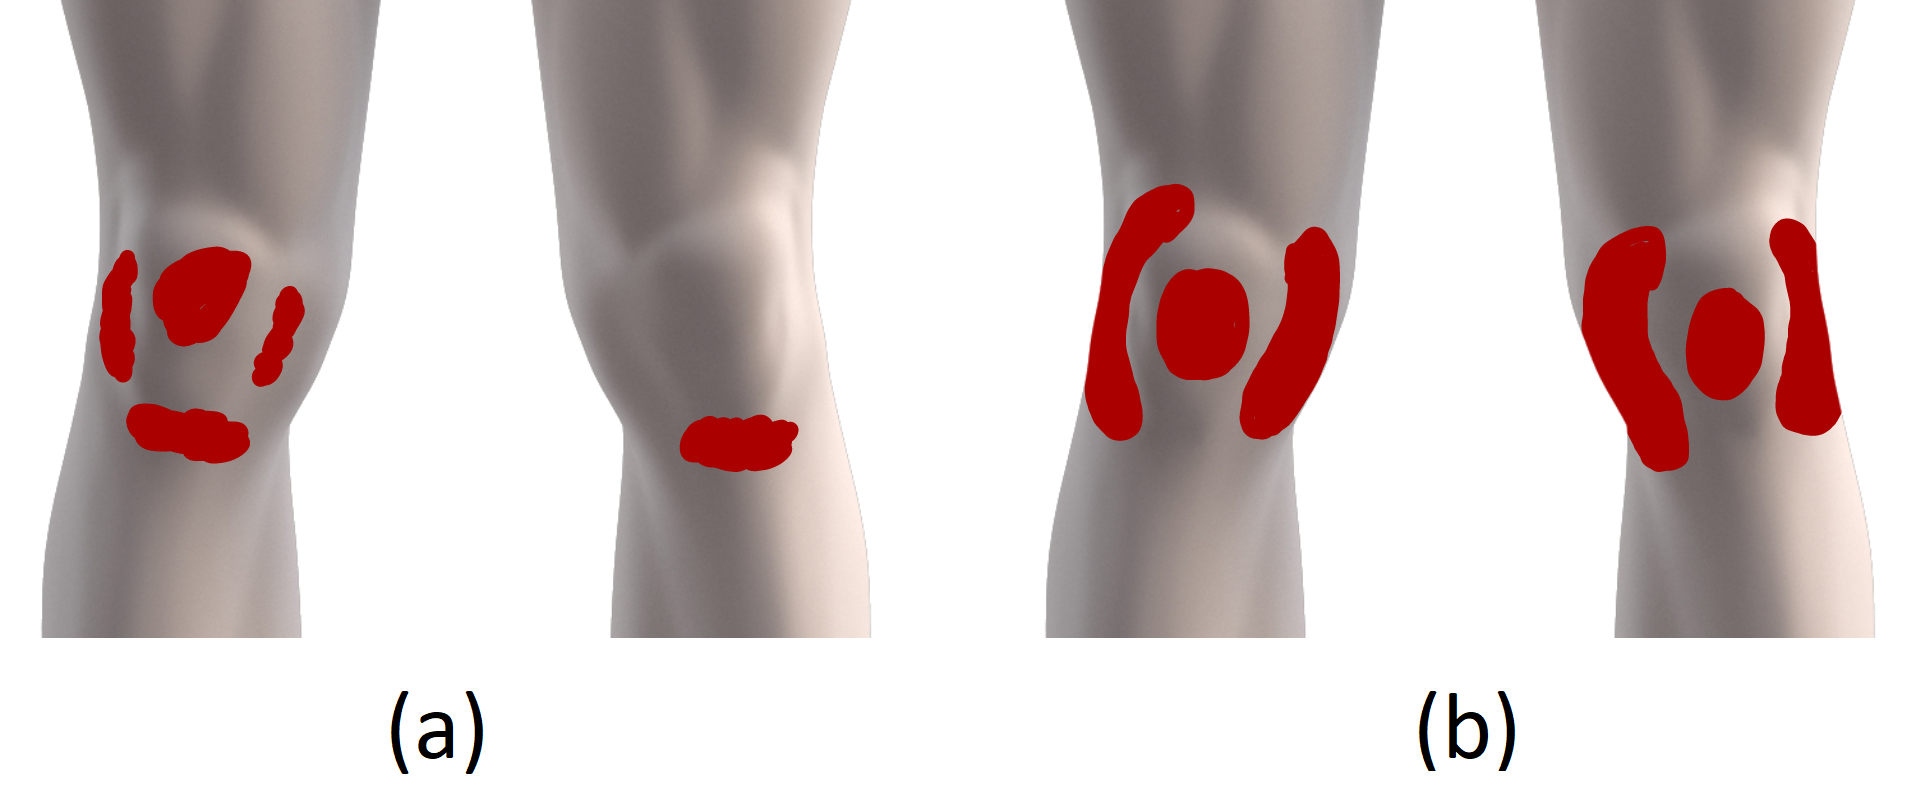
\includegraphics[width=0.46\textwidth]{Figures/Simmetry}
\caption{Pain maps for (a) asymmetric PFP, and (b) symmetric PFP.}
\label{fig:bipainmap}
\end{figure}

\subsection{Classification of pain maps}
The linear correlations showed a poor fit according to the regression line. Thus, the deep learning model did not only use simple features to predict pain duration or pain intensity.
The result showed that the model classifying the CR according to pain intensity had the highest accuracy, whereas the model classifying the LR according to pain duration scored the lowest accuracy. Additionally, the sensitivity and specificity needs to be considered, given that if either sensitivity or specificity is zero valued, the accuracy only reflects the total number of pain maps in one given class.\newline
\noindent
The models including MR, were able to predict according to both lower and higher extremes, which may indicate that there is a pattern to be found in this representation. Additionally, there is a indication of more patterns to be found in the higher extremes. This may support  the finding in the study by \citeauthor{Boudreau2017} \citep{Boudreau2017}, showing a partial correlation between pain maps and pain duration or pain intensity for individuals with PFP longer than five years.
The result of the models using the LR could not distinguish between the pain maps according to the extremes for both pain duration and pain intensity. The models simply classified all pain maps as being in the higher classes, suggesting/indicating that no patterns are learned for the lower extreme classifications, for both pain duration and pain intensity. It can be as a result of the simplified representation of the location, which did not present the size of the pain, only the active region.
The models using the CR resulted in the highest performance when predicting pain intensity, according to the accuracy, sensitivity and specificity. This may be a result of more patterns to be found in the CR, because it includes features from both the morphology and location of the pain. 
Overall, the models performed better when classifying higher intervals, which might be reflected as a result of the imbalance of the pain maps with lower and higher pain durations or pain intensities. This imbalance can be seen in Table \ref{tab:painmaps}, where the higher classes contain more pain maps.
It can be discussed that, the models predicting pain duration according to MR had the highest accuracy, suggesting that the MR may contain more beneficial features for predicting according to pain duration than pain intensity. However, pain intensity had a higher predictive value in relation to CR, than pain duration, which may be a result of CR having more beneficial features to predict pain intensity. 
The performance accuracy, obtained when using LR, shows that it had the lowest performance, since it only could predict according to the higher extremes, which makes it the least recommended representation for predicting either pain duration or pain intensity.   

\subsection{Limitation of threshold}
The LR had a 5\% threshold that defined when a pain region was considered active according to the amount of pain. It can be discussed whether this threshold was suitable, since adding the threshold resulted in loss of pain maps that had a very small amount of pain. However, a smaller threshold or no threshold would give active pain regions that might only contain very few pain pixels. Since PFP is described as hard to localize, it is unknown how precise the individuals have drawn their pain, thus every pixel should maybe not be taken into account.
The CR did not have a threshold for defining active pain regions, because the morphology of the pain would be affected when discarding small pain regions. This representation is not a complete combination of the MR and LR. A threshold could be applied for CR as well, to which additional threshold values to preserve the morphology of pain should be explored. 

\subsection{Optimization of deep learning models}
Optimization of the deep learning models is often a time-consuming process based on the picks of the multiple hyperparameters and different algorithms which could be implemented during the development of the models.
Activation functions were chosen based on the literature, where ReLU should be used for convolutional and fully connected layers in neural network models, and sigmoid should be picked for binary output layer. However, additional testing could be made by using softmax or linear activation function to increase the generalization performance. The dropout algorithm was set to the default 0.5 and used in all models between the fully connected layers to turn off the amount of nodes and prevent the models from overfitting. Additional values could have been tested in order to find most optimal for the every model.
Unfortunately, the lack of time and time-consuming reruns during every optimization cycle, lead to use the common hyperparameters as there were many other which were tested with grid search 10-fold cross validation.
\noindent
Additional limitation for this study was the lack of computational power which lead to a more simple architecture of the models, containing less layers and a lower range of hyperparameters. Thus, an improvement in performance may be found through more powerful systems or services. \\
\noindent
A further optimization of the models may be found according to the input parameters, to which more physical, and psychological features may increase the performance accuracy. Physical features, such as age, height, weight, physical activity level, and sport activity, may influence pain duration or pain intensity. Age could be a relevant feature since the perceived pain is dependent on the individual's personality and character. Younger individuals may feel more pain because of a new pain, than older individuals which have had PFP for a longer period of time. In addition, older individuals may feel more pain because of the phenomenon central sensitization, which in some cases may facilitate widespread pain. The physical activity level, and sport may increase the pain intensity for some individuals because of the patellofemoral loaded activity. Psychological factor is an important feature to consider, because of its influence on pain intensity. Pain is multifactorial and can be influenced of psychosocial factors \citep{Roos2003}. Furthermore, other pain areas, such as hip pain, may influence the pain intensity of PFP.


